\documentclass[11pt,a4paper]{article}

% ── Packages ─────────────────────────────────────────────────────────────────
\usepackage[utf8]{inputenc}
\usepackage[T1]{fontenc}
\usepackage{lmodern}
\usepackage[margin=1in]{geometry}
\usepackage{amsmath,amssymb,amsfonts}
\usepackage{graphicx}
\usepackage{booktabs}
\usepackage{hyperref}
\usepackage{cleveref}
\usepackage{algorithm}
\usepackage{algpseudocode}
\usepackage{enumitem}
\usepackage{xcolor}
\usepackage{tikz}
\usetikzlibrary{positioning,arrows.meta,fit,calc,decorations.pathreplacing}

\hypersetup{
    colorlinks=true,
    linkcolor=blue!70!black,
    citecolor=blue!70!black,
    urlcolor=blue!70!black,
}

% ── Macros ───────────────────────────────────────────────────────────────────
\newcommand{\R}{\mathbb{R}}
\newcommand{\bx}{\mathbf{x}}
\newcommand{\bz}{\mathbf{z}}
\newcommand{\bv}{\mathbf{v}}
\newcommand{\bc}{\mathbf{c}}
\newcommand{\bh}{\mathbf{h}}
\newcommand{\bQ}{\mathbf{Q}}
\newcommand{\bK}{\mathbf{K}}
\newcommand{\bV}{\mathbf{V}}
\newcommand{\softmax}{\operatorname{softmax}}
\newcommand{\LayerNorm}{\operatorname{LayerNorm}}
\newcommand{\Linear}{\operatorname{Linear}}
\newcommand{\SiLU}{\operatorname{SiLU}}
\newcommand{\GELU}{\operatorname{GELU}}
\newcommand{\diag}{\operatorname{diag}}

\title{The Diffusion Transformer:\\
A Complete Architectural Description}
\author{Technical Reference}
\date{\today}

% ═════════════════════════════════════════════════════════════════════════════
\begin{document}
\maketitle

% ── Abstract ─────────────────────────────────────────────────────────────────
\begin{abstract}
The Diffusion Transformer (DiT) replaces the U-Net backbone traditionally used
in diffusion and flow-matching models with a transformer operating on sequences
of image patch tokens.  Given an image $\bx \in \R^{C \times H \times W}$ and a
scalar timestep $t \in [0,1]$, the DiT predicts a velocity field
$\bv \in \R^{C_{\text{out}} \times H \times W}$ that drives a flow from one
image distribution to another.  Conditioning on $t$ is achieved through
\emph{adaptive layer normalisation with zero initialisation} (adaLN-Zero),
which modulates each transformer block's internal normalisation statistics
as a learned function of $t$.  This document provides a self-contained,
equation-level description of every component: patch embedding, two-dimensional
sinusoidal positional encoding, sinusoidal timestep embedding, the adaLN-Zero
transformer block (including its attention and MLP sub-layers), the final
projection layer, the unpatchify operation, and the weight initialisation
scheme.  We also situate the architecture in its historical context and survey
its applications.
\end{abstract}

\tableofcontents
\newpage

% ═════════════════════════════════════════════════════════════════════════════
\section{Overview}
\label{sec:overview}

The Diffusion Transformer is a neural network that maps a noisy or
interpolated image (together with a scalar timestep) to a velocity field of
the same spatial dimensions.  At a high level, the forward pass proceeds
through five stages:

\begin{enumerate}[label=\textbf{(\roman*)}]
    \item \textbf{Patchify.}  A strided convolution partitions the input image
          into a grid of non-overlapping patches and linearly projects each
          patch into a $D$-dimensional token embedding.
    \item \textbf{Position embedding.}  A fixed, two-dimensional sinusoidal
          embedding is added to every token so that the transformer can
          distinguish spatial locations.
    \item \textbf{Timestep conditioning.}  The scalar $t$ is mapped through a
          sinusoidal encoding followed by a small MLP to produce a
          $D$-dimensional conditioning vector $\bc$ that is shared across all
          tokens.
    \item \textbf{Transformer block stack.}  The token sequence passes through
          $L$ identical DiT blocks, each containing multi-head self-attention
          and a feed-forward MLP, both gated and modulated by $\bc$ via the
          adaLN-Zero mechanism.
    \item \textbf{Final layer and unpatchify.}  A final adaLN-modulated linear
          projection maps each token to $p^2 \cdot C_{\text{out}}$ values,
          which are reshaped back into a spatial image.
\end{enumerate}

\noindent
The net effect is a function
\begin{equation}
    f_\theta : \R^{C \times H \times W} \times [0,1]
    \;\longrightarrow\;
    \R^{C_{\text{out}} \times H \times W},
    \qquad
    (\bx, t) \mapsto \bv,
\end{equation}
where $\theta$ denotes all learnable parameters.  Both the input and output
are full-resolution images; the patchification is an internal implementation
detail that is reversed before the output is returned.

The architecture is an \emph{isotropic} design: every transformer block
operates at the same spatial resolution and hidden dimension, with no
downsampling or upsampling stages.  This stands in contrast to the multi-scale
hierarchy of U-Nets and gives the DiT a simpler, more uniform computational
structure.

\Cref{fig:architecture} provides a schematic overview.

\begin{figure}[ht]
\centering
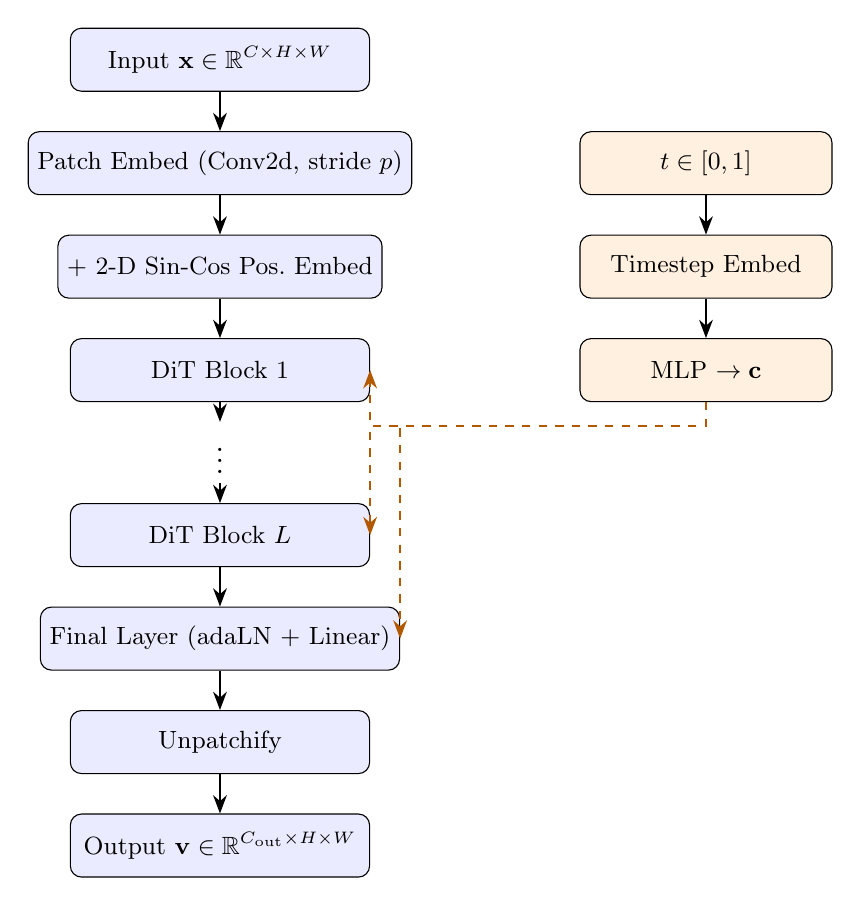
\begin{tikzpicture}[
    >=Stealth,
    block/.style={draw, rounded corners, minimum width=3.8cm, minimum height=0.8cm,
                  fill=blue!8, font=\small},
    cond/.style={draw, rounded corners, minimum width=3.2cm, minimum height=0.8cm,
                 fill=orange!12, font=\small},
    arrow/.style={->, thick},
]
    % Main pipeline
    \node[block] (input)  {Input $\bx \in \R^{C \times H \times W}$};
    \node[block, below=0.5cm of input] (patch) {Patch Embed (Conv2d, stride $p$)};
    \node[block, below=0.5cm of patch] (pos)   {$+$ 2-D Sin-Cos Pos.\ Embed};
    \node[block, below=0.5cm of pos]   (dit1)  {DiT Block $1$};
    \node[below=0.25cm of dit1, font=\large] (dots) {$\vdots$};
    \node[block, below=0.25cm of dots] (ditL)  {DiT Block $L$};
    \node[block, below=0.5cm of ditL]  (final) {Final Layer (adaLN + Linear)};
    \node[block, below=0.5cm of final] (unpatch) {Unpatchify};
    \node[block, below=0.5cm of unpatch] (output) {Output $\bv \in \R^{C_{\text{out}} \times H \times W}$};

    % Conditioning branch
    \node[cond, right=2.5cm of pos]   (temb) {Timestep Embed};
    \node[cond, above=0.5cm of temb]  (tin)  {$t \in [0,1]$};
    \node[cond, below=0.5cm of temb]  (tmlp) {MLP $\to \bc$};

    % Main arrows
    \draw[arrow] (input)   -- (patch);
    \draw[arrow] (patch)   -- (pos);
    \draw[arrow] (pos)     -- (dit1);
    \draw[arrow] (dit1)    -- (dots);
    \draw[arrow] (dots)    -- (ditL);
    \draw[arrow] (ditL)    -- (final);
    \draw[arrow] (final)   -- (unpatch);
    \draw[arrow] (unpatch) -- (output);

    % Conditioning arrows
    \draw[arrow] (tin)  -- (temb);
    \draw[arrow] (temb) -- (tmlp);
    \draw[arrow, dashed, orange!70!black] (tmlp.south) -- ++(0,-0.3) -| ($(dit1.east)+(0,0)$);
    \draw[arrow, dashed, orange!70!black] (tmlp.south) -- ++(0,-0.3) -| ($(ditL.east)+(0,0)$);
    \draw[arrow, dashed, orange!70!black] (tmlp.south) -- ++(0,-0.3) -| ($(final.east)+(0,0)$);
\end{tikzpicture}
\caption{High-level architecture of the Diffusion Transformer.  The main
data path (blue) processes patch tokens through a stack of transformer
blocks.  The conditioning path (orange, dashed) broadcasts the timestep
embedding $\bc$ to every block and to the final layer via adaLN-Zero
modulation.}
\label{fig:architecture}
\end{figure}


% ═════════════════════════════════════════════════════════════════════════════
\section{Background and Prior Work}
\label{sec:background}

\subsection{Denoising Score Matching and Diffusion Models}

Diffusion models~\cite{ho2020denoising,song2021scorebased} learn to reverse a
gradual noising process.  Given data distribution $\pi_1$, a forward process
progressively corrupts samples toward a simple prior (typically Gaussian).
A neural network is trained to predict the score, noise, or velocity at each
noise level, enabling iterative sampling.

\emph{Rectified flow}~\cite{liu2023flow} recasts this as an ODE: the network
learns a velocity field $\bv(\bz_t, t)$ along straight-line interpolations
$\bz_t = t \, \bz_1 + (1-t) \, \bz_0$ between source and target
distributions.  Solving the ODE $d\bz_t = \bv(\bz_t, t)\,dt$ from $t=0$ to
$t=1$ transports samples from $\pi_0$ to $\pi_1$.

\subsection{The U-Net Era}

For most of the history of diffusion models, the velocity (or noise)
prediction network has been a U-Net~\cite{ronneberger2015unet}.  The U-Net's
encoder--decoder structure with skip connections operates at multiple spatial
resolutions, making it naturally suited to dense, pixel-level prediction tasks.
Starting from the DDPM architecture~\cite{ho2020denoising}, the standard recipe
became a U-Net with:

\begin{itemize}[nosep]
    \item Residual blocks at each resolution level,
    \item Self-attention at one or more low-resolution stages,
    \item Timestep conditioning via additive embedding or FiLM
          (Feature-wise Linear Modulation)~\cite{perez2018film},
    \item Downsampling via strided convolutions or average pooling,
          upsampling via bilinear interpolation or transposed convolutions.
\end{itemize}

The U-Net's inductive biases---locality through convolutions, multi-scale
feature hierarchies through down/upsampling, and dense skip connections that
preserve fine spatial detail---made it the dominant architecture for image
generation for several years.  Models such as Stable
Diffusion~\cite{rombach2022latent}, DALL-E~2~\cite{ramesh2022dalle2}, and
Imagen~\cite{saharia2022imagen} all relied on U-Net backbones.

\subsection{Vision Transformers}

The Vision Transformer (ViT)~\cite{dosovitskiy2021vit} demonstrated that a
standard transformer, applied to sequences of image patches, could match or
exceed convolutional networks on image classification at sufficient scale.  ViT
partitions an image into fixed-size patches, linearly embeds each patch into a
token, prepends a learnable \texttt{[CLS]} token, adds learned positional
embeddings, and processes the sequence through a standard transformer encoder.
The \texttt{[CLS]} token's final representation is used for classification.

The key insight was that the transformer's global self-attention, applied to
every pair of patch tokens, provides a powerful mechanism for modelling
long-range spatial dependencies without the locality constraints of
convolutions.  The cost is quadratic in the number of tokens, but for
moderate-resolution images (e.g.\ $224 \times 224$ with patch size 16, giving
196 tokens), this is tractable.

\subsection{From ViT to DiT}

Peebles and Xie~\cite{peebles2023dit} proposed replacing the U-Net with a
transformer backbone, yielding the Diffusion Transformer (DiT).  Their key
contributions were:

\begin{enumerate}[nosep]
    \item Demonstrating that an isotropic transformer (no multi-scale hierarchy)
          could match and surpass U-Net performance on class-conditional
          ImageNet generation.
    \item Introducing \emph{adaLN-Zero} as the conditioning mechanism,
          outperforming alternatives such as cross-attention, in-context
          conditioning, and standard adaptive layer norm.
    \item Showing that DiT obeys \emph{Gflop scaling laws}:
          performance improves smoothly with increased compute, enabling
          predictable scaling.
\end{enumerate}

The DiT architecture was subsequently adopted---with
variations---by Stable Diffusion~3~\cite{esser2024sd3} (as the MMDiT) and
FLUX~\cite{flux2024}, establishing it as the successor to U-Nets for
state-of-the-art image generation.


% ═════════════════════════════════════════════════════════════════════════════
\section{Architecture in Detail}
\label{sec:architecture}

We now describe every component of the DiT in full mathematical detail.
Throughout, let $B$ denote the batch size, $C$ the input channels,
$C_{\text{out}}$ the output channels, $H$ and $W$ the spatial dimensions,
$p$ the patch size, $D$ the hidden (model) dimension,
$N_h$ the number of attention heads, $d_h = D / N_h$ the head dimension,
and $L$ the number of transformer blocks.


% ─────────────────────────────────────────────────────────────────────────────
\subsection{The DiT Forward Pass}
\label{sec:dit-forward}

\Cref{alg:dit-forward} summarises the complete forward pass.  The subsections
that follow describe each step in detail.

\begin{algorithm}[ht]
\caption{DiT Forward Pass}
\label{alg:dit-forward}
\begin{algorithmic}[1]
\Require Image $\bx \in \R^{B \times C \times H \times W}$,
         timestep $t \in \R^{B}$ with $t_i \in [0,1]$
\Ensure  Velocity $\bv \in \R^{B \times C_{\text{out}} \times H \times W}$
\State $\bx \gets \textsc{PatchEmbed}(\bx)$
    \Comment{\texttt{self.x\_embedder(x)} $\;\to (B, D, H', W')$}
\State $\bx \gets \textsc{Flatten}(\bx)$
    \Comment{\texttt{x.flatten(2).transpose(1, 2)} $\;\to (B, T, D)$}
\State $\bx \gets \bx + \textsc{PosEmbed2D}(H', W')$
    \Comment{\texttt{x + self.\_cached\_pos\_emb.unsqueeze(0)}}
\State $\bc \gets \textsc{TimestepMLP}(\textsc{SinCosEmbed}(t))$
    \Comment{\texttt{self.t\_embedder(get\_timestep\_embedding(t, D))}}
\For{$\ell = 1, \ldots, L$}
    \State $\bx \gets \textsc{DiTBlock}_\ell(\bx, \bc)$
    \Comment{\texttt{block(x, c)}}
\EndFor
\State $\bx \gets \textsc{FinalLayer}(\bx, \bc)$
    \Comment{\texttt{self.final\_layer(x, c)} $\;\to (B, T, p^2 C_{\text{out}})$}
\State $\bv \gets \textsc{Unpatchify}(\bx, H', W')$
    \Comment{\texttt{self.unpatchify(x, Hp, Wp)} $\;\to (B, C_{\text{out}}, H, W)$}
\State \Return $\bv$
\end{algorithmic}
\end{algorithm}


% ─── 3.1.1 Patchify ─────────────────────────────────────────────────────────
\subsubsection{Patch Embedding}
\label{sec:patchify}

The input image $\bx \in \R^{C \times H \times W}$ is partitioned into a grid
of $H' \times W'$ non-overlapping patches, where $H' = H/p$ and $W' = W/p$.
Each patch is a $C \times p \times p$ tensor.  A \texttt{Conv2d} with kernel
size $p$ and stride $p$ jointly extracts and linearly projects all patches:
\begin{equation}
    \mathbf{E} = \texttt{Conv2d}(\bx; \; W_e \in \R^{D \times C \times p \times p},
                                  \; b_e \in \R^{D})
    \;\in\; \R^{D \times H' \times W'}.
\end{equation}
This is mathematically equivalent to flattening each $C \times p \times p$
patch into a vector of length $Cp^2$ and multiplying by a weight matrix
$W \in \R^{D \times Cp^2}$, but the strided convolution is computationally
more efficient and avoids explicit reshaping.

The result is flattened to a sequence:
$\mathbf{E} \in \R^{D \times H' \times W'} \to \R^{T \times D}$
where $T = H' W'$ is the sequence length (number of patch tokens).


% ─── 3.1.2 Positional Embedding ─────────────────────────────────────────────
\subsubsection{Two-Dimensional Sinusoidal Positional Embedding}
\label{sec:posembed}

Since self-attention is permutation-equivariant, explicit positional
information must be injected.  The DiT uses fixed (non-learned) 2-D sinusoidal
embeddings that separately encode the row and column coordinates of each patch.

The embedding dimension $D$ is split in half: $D/2$ dimensions for the vertical
axis (rows) and $D/2$ for the horizontal axis (columns).  For each axis, the
encoding follows the Transformer sinusoidal schedule~\cite{vaswani2017attention}.
Let $d = D/4$ be the number of frequency bands per axis.  The frequency for
band $i$ is:
\begin{equation}
    \omega_i = \frac{1}{10000^{\;i / d}},
    \qquad i = 0, 1, \ldots, d-1.
\end{equation}

For a patch at grid position $(r, c)$ where $0 \le r < H'$ and $0 \le c < W'$,
the row embedding occupies the first $D/2$ dimensions:
\begin{equation}
    \mathbf{p}_{\text{row}}(r) =
    \bigl[\,
        \sin(r \omega_0),\; \ldots,\; \sin(r \omega_{d-1}),\;
        \cos(r \omega_0),\; \ldots,\; \cos(r \omega_{d-1})
    \,\bigr]
    \;\in\; \R^{D/2},
\end{equation}
and the column embedding occupies the last $D/2$ dimensions:
\begin{equation}
    \mathbf{p}_{\text{col}}(c) =
    \bigl[\,
        \sin(c \omega_0),\; \ldots,\; \sin(c \omega_{d-1}),\;
        \cos(c \omega_0),\; \ldots,\; \cos(c \omega_{d-1})
    \,\bigr]
    \;\in\; \R^{D/2}.
\end{equation}

The full positional embedding for patch $(r,c)$ is their concatenation:
\begin{equation}
    \mathbf{p}(r,c) =
    \bigl[\, \mathbf{p}_{\text{row}}(r) \;\|\; \mathbf{p}_{\text{col}}(c) \,\bigr]
    \;\in\; \R^{D},
\end{equation}
which is added element-wise to the patch token: $\bx_{r,c} \gets \bx_{r,c} + \mathbf{p}(r,c)$.

Because the embedding is computed analytically from the grid dimensions, it
requires no learned parameters, generalises to arbitrary resolutions (the
embedding is recomputed and cached whenever the resolution changes), and
encodes 2-D spatial structure explicitly rather than relying on the model to
infer it from a 1-D ordering.


% ─── 3.1.3 Timestep Conditioning ────────────────────────────────────────────
\subsubsection{Timestep Conditioning}
\label{sec:timestep}

The scalar timestep $t \in [0,1]$ must be mapped to a high-dimensional
representation before it can usefully condition the network.  This happens in
two stages.

\paragraph{Stage 1: Sinusoidal encoding.}
Following~\cite{ho2020denoising}, which in turn follows~\cite{vaswani2017attention},
the scalar $t$ is mapped to a $D$-dimensional vector using sinusoidal features.
Let $d = D/2$ and define frequency bands:
\begin{equation}
    \omega_i = \exp\!\bigl(-i \cdot \ln(10000) / (d - 1)\bigr),
    \qquad i = 0, \ldots, d-1.
\end{equation}

The raw encoding is:
\begin{equation}
    \textsc{SinCosEmbed}(t) =
    \bigl[\,
        \sin(1000 \cdot t \cdot \omega_0),\; \ldots,\; \sin(1000 \cdot t \cdot \omega_{d-1}),\;
        \cos(1000 \cdot t \cdot \omega_0),\; \ldots,\; \cos(1000 \cdot t \cdot \omega_{d-1})
    \,\bigr]
    \;\in\; \R^{D}.
    \label{eq:sincos-t}
\end{equation}

The factor of $1000$ rescales the $[0,1]$ timestep range to
$[0,1000]$, matching the scale used by DDPM's integer timestep
convention~\cite{ho2020denoising}.  Without this rescaling, the
high-frequency bands would see only a tiny fraction of one period across the
full timestep range, producing nearly-constant features and wasting
representational capacity.

This sinusoidal encoding is a \emph{Fourier feature map}: it lifts the scalar
$t$ into a space where subsequent linear layers can represent arbitrary smooth
functions of $t$, overcoming the limitation that a linear layer applied
directly to a scalar can only learn an affine function.

\paragraph{Stage 2: Learnable MLP.}
The sinusoidal features are passed through a two-layer MLP with SiLU
activation:
\begin{equation}
    \bc = W_2 \,\SiLU(W_1 \,\textsc{SinCosEmbed}(t) + b_1) + b_2
    \;\in\; \R^{D},
\end{equation}
where $W_1 \in \R^{4D \times D}$, $b_1 \in \R^{4D}$,
$W_2 \in \R^{D \times 4D}$, $b_2 \in \R^{D}$.  The intermediate expansion to
$4D$ (a \emph{bottleneck ratio} of 4) provides ample capacity for the network
to learn a rich, nonlinear function of timestep.

The resulting conditioning vector $\bc$ is shared by all tokens in a given
sample and broadcast to every DiT block and the final layer.


% ─── 3.1.4 Transformer Block Stack ──────────────────────────────────────────
\subsubsection{Transformer Block Stack}
\label{sec:blockstack}

The token sequence is processed by $L$ identical DiT blocks in series:
\begin{equation}
    \bx^{(\ell)} = \textsc{DiTBlock}_\ell\!\bigl(\bx^{(\ell-1)}, \bc\bigr),
    \qquad \ell = 1, \ldots, L,
\end{equation}
where $\bx^{(0)}$ is the position-encoded patch embedding and each block has
its own learnable parameters.  The conditioning vector $\bc$ is the same for
all blocks---it is computed once and reused.

The stack is \emph{isotropic}: every block operates at the same hidden
dimension $D$ and the same sequence length $T$.  There is no spatial
downsampling, no pooling, and no multi-scale hierarchy.  All spatial mixing
occurs through self-attention.


% ─── 3.1.5 Final Layer and Unpatchify ────────────────────────────────────────
\subsubsection{Final Layer and Unpatchify}
\label{sec:finallayer}

After the last transformer block, the token sequence must be mapped back to
pixel space.

\paragraph{Final layer.}
The final layer applies adaLN modulation (shift and scale only, no gate)
followed by a linear projection.  Given the conditioning vector $\bc$:
\begin{align}
    (\boldsymbol{\beta}_f,\; \boldsymbol{\gamma}_f)
    &= \textsc{Split}\!\bigl(\Linear(\SiLU(\bc))\bigr),
    \quad \boldsymbol{\beta}_f, \boldsymbol{\gamma}_f \in \R^{D}
    \\[4pt]
    \hat{\bx} &= (1 + \boldsymbol{\gamma}_f) \odot \LayerNorm(\bx) + \boldsymbol{\beta}_f
    \\[4pt]
    \bx_{\text{out}} &= W_f \,\hat{\bx} + b_f,
    \quad W_f \in \R^{(p^2 C_{\text{out}}) \times D},\; b_f \in \R^{p^2 C_{\text{out}}}.
\end{align}

Each token is now a vector of length $p^2 C_{\text{out}}$, encoding all output
channels for all pixels within one patch.

Note that the final layer uses only shift and scale (2 modulation vectors)
rather than the 6 vectors (shift, scale, gate $\times$ 2) used in the main
blocks.  There is no gate because the final layer's output is used directly,
not added as a residual.

\paragraph{Unpatchify.}
The output tokens are reshaped from $(B, T, p^2 C_{\text{out}})$ back to a
spatial image $(B, C_{\text{out}}, H, W)$ by the inverse of the patchification:
\begin{equation}
    \R^{B \times T \times p^2 C_{\text{out}}}
    \;\xrightarrow{\text{reshape}}\;
    \R^{B \times H' \times W' \times p \times p \times C_{\text{out}}}
    \;\xrightarrow{\text{permute}}\;
    \R^{B \times C_{\text{out}} \times H \times W}.
\end{equation}

The permutation interleaves the patch-internal pixel coordinates with the
patch grid coordinates, reconstructing the original spatial layout:
$(B, H', W', p, p, C_{\text{out}}) \to (B, C_{\text{out}}, H', p, W', p) \to (B, C_{\text{out}}, H, W)$.


% ─────────────────────────────────────────────────────────────────────────────
\subsection{The DiT Block}
\label{sec:ditblock}

Each DiT block is a pre-norm transformer block with two sub-layers---multi-head
self-attention (MSA) and a feed-forward MLP---both modulated and gated by the
timestep conditioning vector $\bc$.  \Cref{fig:ditblock} shows the block's
internal structure.

\begin{figure}[ht]
\centering
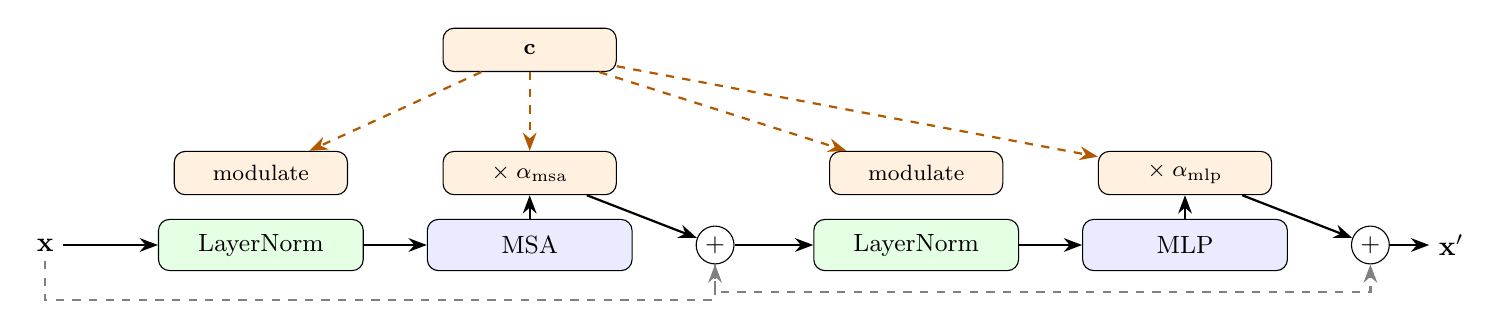
\begin{tikzpicture}[
    >=Stealth,
    block/.style={draw, rounded corners, minimum width=2.6cm, minimum height=0.65cm,
                  fill=blue!8, font=\small},
    norm/.style={draw, rounded corners, minimum width=2.6cm, minimum height=0.65cm,
                 fill=green!10, font=\small},
    cond/.style={draw, rounded corners, minimum width=2.2cm, minimum height=0.55cm,
                 fill=orange!12, font=\footnotesize},
    op/.style={draw, circle, inner sep=1.5pt, font=\small},
    arrow/.style={->, thick},
]
    % Input
    \node (xin) {$\bx$};

    % Attention path
    \node[norm, right=1.2cm of xin] (norm1) {LayerNorm};
    \node[cond, above=0.3cm of norm1] (mod1) {modulate};
    \node[block, right=0.8cm of norm1] (msa) {MSA};
    \node[cond, above=0.3cm of msa] (gate1) {$\times\; \alpha_{\text{msa}}$};
    \node[op, right=0.8cm of msa] (add1) {$+$};

    % MLP path
    \node[norm, right=1.0cm of add1] (norm2) {LayerNorm};
    \node[cond, above=0.3cm of norm2] (mod2) {modulate};
    \node[block, right=0.8cm of norm2] (mlp) {MLP};
    \node[cond, above=0.3cm of mlp] (gate2) {$\times\; \alpha_{\text{mlp}}$};
    \node[op, right=0.8cm of mlp] (add2) {$+$};

    % Output
    \node[right=0.5cm of add2] (xout) {$\bx'$};

    % Main flow
    \draw[arrow] (xin) -- (norm1);
    \draw[arrow] (norm1) -- (msa);
    \draw[arrow] (msa) -- (gate1);
    \draw[arrow] (gate1) -- (add1);
    \draw[arrow] (add1) -- (norm2);
    \draw[arrow] (norm2) -- (mlp);
    \draw[arrow] (mlp) -- (gate2);
    \draw[arrow] (gate2) -- (add2);
    \draw[arrow] (add2) -- (xout);

    % Skip connections
    \draw[arrow, gray, dashed] (xin.south) -- ++(0,-0.5) -| (add1.south);
    \draw[arrow, gray, dashed] (add1.south) -- ++(0,-0.35) -| (add2.south);

    % Conditioning
    \node[cond, above=1.0cm of gate1] (c) {$\bc$};
    \draw[arrow, orange!70!black, dashed] (c) -- (mod1);
    \draw[arrow, orange!70!black, dashed] (c) -- (gate1);
    \draw[arrow, orange!70!black, dashed] (c) -- (mod2);
    \draw[arrow, orange!70!black, dashed] (c) -- (gate2);

\end{tikzpicture}
\caption{Internal structure of a DiT block.  Grey dashed arrows show residual
connections.  Orange dashed arrows show the flow of the conditioning vector
$\bc$, which controls both the modulation of normalisation and the gating of
sub-layer outputs.}
\label{fig:ditblock}
\end{figure}


% ─── DiTBlock pseudocode ─────────────────────────────────────────────────────
\Cref{alg:ditblock-forward} gives the complete DiTBlock forward pass as
pseudocode.  Every line corresponds directly to a line in the Python
implementation; the right column shows the Python variable name used in
\texttt{DiTBlock.forward()}.

\begin{algorithm}[ht]
\caption{DiTBlock Forward Pass}
\label{alg:ditblock-forward}
\begin{algorithmic}[1]
\Require Tokens $\bx \in \R^{B \times T \times D}$,
         conditioning $\bc \in \R^{B \times D}$
\Ensure  Updated tokens $\bx' \in \R^{B \times T \times D}$
\State $(\boldsymbol{\beta}_1, \boldsymbol{\gamma}_1, \boldsymbol{\alpha}_1,
         \boldsymbol{\beta}_2, \boldsymbol{\gamma}_2, \boldsymbol{\alpha}_2)
       \gets \textsc{Chunk}_6\!\bigl(\Linear(\SiLU(\bc))\bigr)$
    \Comment{\texttt{shift\_msa, scale\_msa, gate\_msa, shift\_mlp, scale\_mlp, gate\_mlp}}
\Statex \hspace{\algorithmicindent}\textit{--- Attention path ---}
\State $\hat{\bx} \gets (1 + \boldsymbol{\gamma}_1) \odot \LayerNorm(\bx) + \boldsymbol{\beta}_1$
    \Comment{\texttt{modulate(self.norm1(x), shift\_msa, scale\_msa)}}
\State $[\bQ \,\|\, \bK \,\|\, \bV] \gets \hat{\bx}\,W_{qkv}^\top + b_{qkv}$
    \Comment{\texttt{self.qkv(h)}}
\State Reshape to $(B, N_h, T, d_h)$ per query/key/value
    \Comment{\texttt{reshape + permute + unbind}}
\State $\bh \gets \textsc{SDPA}(\bQ, \bK, \bV)$
    \Comment{\texttt{F.scaled\_dot\_product\_attention(q, k, v)}}
\State $\bh \gets \bh\,W_O^\top + b_O$
    \Comment{\texttt{self.attn\_out(h)}}
\State $\bx \gets \bx + \boldsymbol{\alpha}_1 \odot \bh$
    \Comment{\texttt{x + gate\_msa.unsqueeze(1) * h}}
\Statex \hspace{\algorithmicindent}\textit{--- MLP path ---}
\State $\hat{\bx} \gets (1 + \boldsymbol{\gamma}_2) \odot \LayerNorm(\bx) + \boldsymbol{\beta}_2$
    \Comment{\texttt{modulate(self.norm2(x), shift\_mlp, scale\_mlp)}}
\State $\bh \gets W_2\,\GELU(W_1\,\hat{\bx} + b_1) + b_2$
    \Comment{\texttt{self.mlp(h)}}
\State $\bx \gets \bx + \boldsymbol{\alpha}_2 \odot \bh$
    \Comment{\texttt{x + gate\_mlp.unsqueeze(1) * h}}
\State \Return $\bx$
\end{algorithmic}
\end{algorithm}

\Cref{tab:notation-mapping} provides a complete mapping between the
mathematical notation used in this paper and the Python variable names in
\texttt{fnn.py}.

\begin{table}[ht]
\centering
\caption{Notation-to-code mapping for DiT and DiTBlock.}
\label{tab:notation-mapping}
\begin{tabular}{@{}lll@{}}
\toprule
\textbf{Paper} & \textbf{Python} & \textbf{Description} \\
\midrule
$\boldsymbol{\beta}_1$ & \texttt{shift\_msa} & Attention pre-norm additive bias \\
$\boldsymbol{\gamma}_1$ & \texttt{scale\_msa} & Attention pre-norm multiplicative scale \\
$\boldsymbol{\alpha}_1$ & \texttt{gate\_msa} & Attention output gate \\
$\boldsymbol{\beta}_2$ & \texttt{shift\_mlp} & MLP pre-norm additive bias \\
$\boldsymbol{\gamma}_2$ & \texttt{scale\_mlp} & MLP pre-norm multiplicative scale \\
$\boldsymbol{\alpha}_2$ & \texttt{gate\_mlp} & MLP output gate \\
$\boldsymbol{\beta}_f$ & \texttt{shift} (final layer) & Final layer pre-norm additive bias \\
$\boldsymbol{\gamma}_f$ & \texttt{scale} (final layer) & Final layer pre-norm multiplicative scale \\
$\bc$ & \texttt{c} & Timestep conditioning vector \\
$D$ & \texttt{hidden\_size} & Model width \\
$N_h$ & \texttt{num\_heads} & Number of attention heads \\
$d_h$ & \texttt{head\_dim} & Per-head dimension ($D / N_h$) \\
$L$ & \texttt{depth} & Number of DiT blocks \\
$r$ & \texttt{mlp\_ratio} & MLP expansion factor \\
$p$ & \texttt{patch\_size} & Patch tokenisation stride \\
\bottomrule
\end{tabular}
\end{table}


% ─── 3.2.1 adaLN-Zero ───────────────────────────────────────────────────────
\subsubsection{Adaptive Layer Normalisation with Zero Initialisation (adaLN-Zero)}
\label{sec:adaln}

Standard Layer Normalisation~\cite{ba2016layernorm} normalises each token to
zero mean and unit variance, then applies a \emph{fixed} learned affine
transformation (scale $\gamma$ and shift $\beta$).  In the DiT, the affine
parameters are not fixed---they are \emph{regressed from the conditioning
vector} $\bc$, making them input-dependent.  This is the ``adaptive'' part.

Each DiT block contains a single modulation network that takes $\bc$ and
produces all six modulation vectors at once:
\begin{equation}
    (\boldsymbol{\beta}_1,\, \boldsymbol{\gamma}_1,\, \boldsymbol{\alpha}_1,\,
     \boldsymbol{\beta}_2,\, \boldsymbol{\gamma}_2,\, \boldsymbol{\alpha}_2)
    = \textsc{Split}\!\bigl(\Linear(\SiLU(\bc))\bigr),
    \label{eq:adaln-regression}
\end{equation}
where each vector $\in \R^D$ and $\Linear : \R^D \to \R^{6D}$.  The vectors
serve the following roles:

\begin{center}
\begin{tabular}{@{}lll@{}}
\toprule
\textbf{Vector} & \textbf{Role} & \textbf{Applied to} \\
\midrule
$\boldsymbol{\beta}_1$ (shift) & additive bias after norm & attention sub-layer \\
$\boldsymbol{\gamma}_1$ (scale) & multiplicative scale after norm & attention sub-layer \\
$\boldsymbol{\alpha}_1$ (gate) & multiplicative gate on output & attention sub-layer \\
$\boldsymbol{\beta}_2$ (shift) & additive bias after norm & MLP sub-layer \\
$\boldsymbol{\gamma}_2$ (scale) & multiplicative scale after norm & MLP sub-layer \\
$\boldsymbol{\alpha}_2$ (gate) & multiplicative gate on output & MLP sub-layer \\
\bottomrule
\end{tabular}
\end{center}

The ``Zero'' in adaLN-Zero refers to the initialisation: the linear layer
in~\cref{eq:adaln-regression} has both its weight matrix and bias vector
initialised to zero.  This means that at the start of training:
\begin{itemize}[nosep]
    \item $\boldsymbol{\gamma} = \mathbf{0}$, so $(1 + \boldsymbol{\gamma}) = \mathbf{1}$
          (identity scale),
    \item $\boldsymbol{\beta} = \mathbf{0}$ (no shift),
    \item $\boldsymbol{\alpha} = \mathbf{0}$ (gate is closed).
\end{itemize}

Because the gate $\boldsymbol{\alpha}$ starts at zero, the residual connection
$\bx + \boldsymbol{\alpha} \odot f(\bx)$ reduces to $\bx + \mathbf{0} = \bx$.
Every block is initially an identity function, and the entire DiT outputs
$\bv = \mathbf{0}$ (since the final layer's projection is also zero-initialised).
Training gradually ``opens'' the gates, allowing each block to contribute.
This is a critical stability mechanism, particularly for deep models.


% ─── 3.2.2 The Modulate Operation ───────────────────────────────────────────
\subsubsection{The Modulate Operation}
\label{sec:modulate}

The \texttt{modulate} function applies the adaptive shift and scale to a
normalised token sequence:
\begin{equation}
    \textsc{Modulate}(\bx, \boldsymbol{\beta}, \boldsymbol{\gamma})
    = (1 + \boldsymbol{\gamma}) \odot \bx + \boldsymbol{\beta},
    \label{eq:modulate}
\end{equation}
where $\bx \in \R^{B \times T \times D}$ and $\boldsymbol{\gamma},
\boldsymbol{\beta} \in \R^{B \times D}$ are broadcast over the token
dimension~$T$.

This is the mechanism by which the timestep controls the transformer's
behaviour.  Standard LayerNorm normalises all tokens to a common distribution
with fixed statistics.  The \texttt{modulate} operation then re-scales and
re-centres them according to the timestep, so the same input image produces
different internal representations at different points along the flow
trajectory.

The $(1 + \boldsymbol{\gamma})$ formulation (rather than just
$\boldsymbol{\gamma}$) is deliberate: when $\boldsymbol{\gamma} = \mathbf{0}$
(as at initialisation), the scale is exactly $\mathbf{1}$ rather than
$\mathbf{0}$, preventing the signal from being annihilated before training
begins.

Note that the LayerNorm used here has \texttt{elementwise\_affine=False},
meaning it has no learned $\gamma$ or $\beta$ parameters of its own.  It also
uses $\varepsilon = 10^{-6}$ (rather than PyTorch's default $10^{-5}$) for
numerical stability.  The
adaptive modulation entirely replaces the standard affine transform, providing
a strictly more expressive alternative: the normalisation statistics are
per-sample and timestep-dependent rather than fixed.


% ─── 3.2.3 Multi-Head Self-Attention ────────────────────────────────────────
\subsubsection{Multi-Head Self-Attention}
\label{sec:attention}

After modulation, the normalised token sequence is projected to queries, keys,
and values via a single fused linear projection:
\begin{equation}
    [\bQ \,\|\, \bK \,\|\, \bV] = \hat{\bx} \, W_{qkv}^{\!\top} + b_{qkv},
    \qquad W_{qkv} \in \R^{3D \times D},\; b_{qkv} \in \R^{3D}.
\end{equation}

The concatenated result is reshaped into $N_h$ heads, each of dimension
$d_h = D / N_h$:
\begin{equation}
    \bQ, \bK, \bV \;\in\; \R^{B \times N_h \times T \times d_h}.
\end{equation}

Attention is computed using \emph{scaled dot-product attention}%
~\cite{vaswani2017attention}:
\begin{equation}
    \textsc{Attention}(\bQ, \bK, \bV) =
    \softmax\!\left(\frac{\bQ \bK^\top}{\sqrt{d_h}}\right) \bV
    \;\in\; \R^{B \times N_h \times T \times d_h}.
    \label{eq:sdpa}
\end{equation}

The $1/\sqrt{d_h}$ scaling prevents the dot products from growing with head
dimension, keeping the softmax in a regime where gradients are well-behaved.
In practice, this computation is delegated to PyTorch's
\texttt{F.scaled\_dot\_product\_attention}, which automatically selects the
most efficient implementation available (FlashAttention~\cite{dao2022flash},
memory-efficient attention, or the mathematical fallback).

The multi-head outputs are concatenated and projected through a linear
output layer:
\begin{equation}
    \bh_{\text{attn}} = \textsc{Concat}(\text{head}_1, \ldots, \text{head}_{N_h}) \, W_O^\top + b_O,
    \qquad W_O \in \R^{D \times D}.
\end{equation}

Finally, the gated residual connection is applied:
\begin{equation}
    \bx \gets \bx + \boldsymbol{\alpha}_1 \odot \bh_{\text{attn}},
\end{equation}
where $\boldsymbol{\alpha}_1 \in \R^{B \times D}$ is broadcast over $T$.
Because the attention sub-layer sees all $T$ tokens simultaneously, this is
where spatial information is mixed globally: every patch can attend to every
other patch, regardless of spatial distance.


% ─── 3.2.4 Feed-Forward MLP ─────────────────────────────────────────────────
\subsubsection{Feed-Forward MLP}
\label{sec:mlp}

After attention, the tokens pass through a position-wise feed-forward network.
The MLP is preceded by its own modulated normalisation:
\begin{align}
    \hat{\bx} &= \textsc{Modulate}\!\bigl(\LayerNorm(\bx),\; \boldsymbol{\beta}_2,\; \boldsymbol{\gamma}_2\bigr), \\[4pt]
    \bh_{\text{mlp}} &= W_2 \,\GELU(W_1 \, \hat{\bx} + b_1) + b_2,
\end{align}
where $W_1 \in \R^{D_{\text{ff}} \times D}$, $W_2 \in \R^{D \times D_{\text{ff}}}$,
and $D_{\text{ff}} = \lfloor r \cdot D \rfloor$ with $r$ being the MLP ratio
(typically $r = 4$, so $D_{\text{ff}} = 4D$).

The GELU activation~\cite{hendrycks2016gelu} is used with the $\tanh$
approximation:
\begin{equation}
    \GELU(x) \approx \frac{x}{2}\left(1 + \tanh\!\left[\sqrt{\frac{2}{\pi}}\left(x + 0.044715\,x^3\right)\right]\right).
\end{equation}

The MLP expands the representation to $4\times$ the hidden dimension, applies
the nonlinearity, and projects back.  Unlike attention, the MLP operates on
each token independently---it performs no inter-token communication.  It serves
as a per-position nonlinear feature transform.

The gated residual is then applied:
\begin{equation}
    \bx \gets \bx + \boldsymbol{\alpha}_2 \odot \bh_{\text{mlp}}.
\end{equation}


% ─────────────────────────────────────────────────────────────────────────────
\subsection{Weight Initialisation}
\label{sec:init}

The initialisation scheme is designed to ensure that the DiT begins training
as a well-conditioned near-identity function.

\begin{enumerate}[nosep]
    \item \textbf{All linear layers:} Xavier uniform initialisation for weights;
          biases set to zero.
    \item \textbf{Patch embedding} (\texttt{Conv2d}): The weight tensor is
          reshaped to 2-D and initialised with Xavier uniform.  Bias set to zero.
    \item \textbf{Timestep MLP:} Weights initialised with
          $\mathcal{N}(0, 0.02^2)$ (small normal), following GPT-2
          convention~\cite{radford2019gpt2}.
    \item \textbf{adaLN modulation layers} (in every block): Both weight and
          bias initialised to zero.  This is the critical ``Zero'' in
          adaLN-Zero---it ensures all gates start closed and all affine
          modulations start as identity.
    \item \textbf{Final layer:} The adaLN modulation, the output linear
          projection weight, and the output bias are all initialised to zero.
          This guarantees $\bv = \mathbf{0}$ at initialisation.
\end{enumerate}

The net effect is that the untrained DiT maps every input to the zero velocity
field: $f_\theta(\bx, t) = \mathbf{0}$ for all $\bx, t$.  This is a
reasonable prior for flow-matching, where the model must learn to predict
velocities that are initially unknown.  Starting from zero is preferable to
starting from random noise, as it avoids large initial losses and gradient
spikes.


% ─────────────────────────────────────────────────────────────────────────────
\subsection{Summary of Hyperparameters}
\label{sec:hyperparams}

\Cref{tab:hyperparams} collects the architectural hyperparameters and their
effects on model capacity and computation.

\begin{table}[ht]
\centering
\caption{DiT architectural hyperparameters.}
\label{tab:hyperparams}
\begin{tabular}{@{}llp{6.5cm}@{}}
\toprule
\textbf{Symbol} & \textbf{Name} & \textbf{Effect} \\
\midrule
$C$, $C_{\text{out}}$ & channels & Input/output image channels (e.g.\ 3 for RGB) \\
$p$ & \texttt{patch\_size} & Patch tokenisation stride; sequence length $T = HW/p^2$ \\
$D$ & \texttt{hidden\_size} & Width of all token representations throughout the network \\
$L$ & \texttt{depth} & Number of DiT blocks; primary control for model capacity \\
$N_h$ & \texttt{num\_heads} & Number of attention heads; must divide $D$ \\
$r$ & \texttt{mlp\_ratio} & MLP hidden dimension as a multiple of $D$ \\
\bottomrule
\end{tabular}
\end{table}

The total parameter count is approximately:
\begin{equation}
    |\theta| \approx
    \underbrace{C p^2 D}_{\text{patch embed}}
    + \underbrace{8D^2}_{\text{timestep MLP}}
    + L \cdot \bigl(
        \underbrace{4D^2}_{\text{QKV + out}}
        + \underbrace{2rD^2}_{\text{MLP}}
        + \underbrace{6D^2 + 6D}_{\text{adaLN mod.}}
    \bigr)
    + \underbrace{p^2 C_{\text{out}} D}_{\text{final layer}},
\end{equation}
which simplifies to $|\theta| \approx L(4 + 2r + 6)D^2 = L(10 + 2r)D^2$ for
the block-dominated term.  With $r = 4$, each block contributes roughly $18D^2$
parameters.  A typical configuration ($D = 768$, $L = 12$, $r = 4$) has
approximately 127 million parameters in the transformer blocks alone.


% ═════════════════════════════════════════════════════════════════════════════
\section{Applications}
\label{sec:applications}

The DiT architecture is a general-purpose conditional image generator: it maps
an input image and a scalar parameter to a same-resolution output.  This
generality enables a wide variety of applications.

\subsection{Diffusion Image Generation}

The original application~\cite{peebles2023dit}: generate images from Gaussian
noise by iteratively integrating the learned velocity field.  Starting from
$\bz_0 \sim \mathcal{N}(\mathbf{0}, \mathbf{I})$, the solver steps
$\bz_{t+\Delta t} = \bz_t + \bv(\bz_t, t) \cdot \Delta t$ from $t=0$ to
$t=1$.  Class conditioning (or text conditioning, as in
SD3~\cite{esser2024sd3}) is typically injected alongside the timestep.

\subsection{Unpaired Image-to-Image Translation}

By setting $\pi_0$ and $\pi_1$ to be two different image domains (e.g.\ horses
and zebras, day and night, sketches and photographs), the DiT learns a velocity
field that transports images from one domain to the other.  When combined with
saliency-weighted flow matching~\cite{liu2023flow}, the network focuses on
transforming domain-relevant features (e.g.\ coat texture) while preserving
domain-invariant structure (e.g.\ pose and background).

\subsection{Image Inpainting}

Given a masked image and a binary mask, the DiT can be conditioned to predict
a velocity field that fills in missing regions.  The input channels are
augmented to include the mask, and the velocity is constrained to be zero in
un-masked regions.  The flow-based formulation naturally handles soft
boundaries.

\subsection{Super-Resolution and Enhancement}

With $\pi_0$ as a distribution of low-resolution (or degraded) images and
$\pi_1$ as high-resolution (or clean) images, the DiT learns to transport
blurry images toward sharp ones.  The patch-based tokenisation is particularly
natural here: the network can attend to both local texture and global structure
simultaneously through self-attention.

\subsection{Style Transfer}

When $\pi_0$ is content images and $\pi_1$ is stylised images, the learned
velocity field performs style transfer.  The saliency network's feature-space
weighting ensures that the flow focuses on style-relevant features (colour
palette, brushwork, texture) rather than content-relevant ones (object
identity, spatial layout).

\subsection{Temporal Prediction and Video}

By extending the patch embedding to a 3-D strided convolution (spatial
$+$ temporal), the DiT can process short video clips as sequences of
spatiotemporal tokens.  The self-attention then captures both spatial
composition and temporal dynamics, enabling applications such as frame
prediction, temporal super-resolution, and video style transfer.

\subsection{Scientific Imaging}

The DiT's ability to learn arbitrary image-to-image transformations makes it
applicable to scientific domains: medical image modality transfer (e.g.\ CT to
MRI), satellite image enhancement, microscopy denoising, and astronomical image
reconstruction.  The saliency-weighted loss is especially useful here, as it
can focus the velocity on scientifically meaningful features.

\subsection{Latent-Space Operation}

When paired with a codec (variational autoencoder or similar), the DiT operates
in a compressed latent space rather than pixel space.  This dramatically
reduces the sequence length (e.g.\ a $128 \times 128$ image with a $4\times$
spatial compression becomes $32 \times 32$ before patchification), enabling
the use of larger models and higher-resolution images within the same
computational budget.  This is the approach taken by Stable
Diffusion~\cite{rombach2022latent} and its successors.


% ═════════════════════════════════════════════════════════════════════════════

\bibliographystyle{unsrt}

\begin{thebibliography}{99}

\bibitem{vaswani2017attention}
A.~Vaswani, N.~Shazeer, N.~Parmar, J.~Uszkoreit, L.~Jones, A.~N.~Gomez,
\L.~Kaiser, and I.~Polosukhin.
\newblock Attention is all you need.
\newblock In \emph{Advances in Neural Information Processing Systems (NeurIPS)}, 2017.

\bibitem{dosovitskiy2021vit}
A.~Dosovitskiy, L.~Beyer, A.~Kolesnikov, D.~Weissenborn, X.~Zhai,
T.~Unterthiner, M.~Dehghani, M.~Minderer, G.~Heigold, S.~Gelly,
J.~Uszkoreit, and N.~Houlsby.
\newblock An image is worth 16x16 words: Transformers for image recognition
  at scale.
\newblock In \emph{International Conference on Learning Representations (ICLR)}, 2021.

\bibitem{ho2020denoising}
J.~Ho, A.~Jain, and P.~Abbeel.
\newblock Denoising diffusion probabilistic models.
\newblock In \emph{Advances in Neural Information Processing Systems (NeurIPS)}, 2020.

\bibitem{song2021scorebased}
Y.~Song, J.~Sohl-Dickstein, D.~P.~Kingma, A.~Kumar, S.~Ermon, and B.~Poole.
\newblock Score-based generative modeling through stochastic differential
  equations.
\newblock In \emph{International Conference on Learning Representations (ICLR)}, 2021.

\bibitem{liu2023flow}
X.~Liu, C.~Gong, and Q.~Liu.
\newblock Flow straight and fast: Learning to generate and transfer data with
  rectified flow.
\newblock In \emph{International Conference on Learning Representations (ICLR)}, 2023.

\bibitem{peebles2023dit}
W.~Peebles and S.~Xie.
\newblock Scalable diffusion models with transformers.
\newblock In \emph{International Conference on Computer Vision (ICCV)}, 2023.

\bibitem{ronneberger2015unet}
O.~Ronneberger, P.~Fischer, and T.~Brox.
\newblock U-Net: Convolutional networks for biomedical image segmentation.
\newblock In \emph{Medical Image Computing and Computer-Assisted Intervention
  (MICCAI)}, 2015.

\bibitem{rombach2022latent}
R.~Rombach, A.~Blattmann, D.~Lorenz, P.~Esser, and B.~Ommer.
\newblock High-resolution image synthesis with latent diffusion models.
\newblock In \emph{IEEE/CVF Conference on Computer Vision and Pattern
  Recognition (CVPR)}, 2022.

\bibitem{ramesh2022dalle2}
A.~Ramesh, P.~Dhariwal, A.~Nichol, C.~Chu, and M.~Chen.
\newblock Hierarchical text-conditional image generation with CLIP latents.
\newblock \emph{arXiv preprint arXiv:2204.06125}, 2022.

\bibitem{saharia2022imagen}
C.~Saharia, W.~Chan, S.~Saxena, L.~Li, J.~Whang, E.~Denton, S.~K.~S.~Ghasemipour,
R.~Gontijo~Lopes, B.~Karagol~Ayan, T.~Salimans, J.~Ho, D.~J.~Fleet, and
M.~Norouzi.
\newblock Photorealistic text-to-image diffusion models with deep language
  understanding.
\newblock In \emph{Advances in Neural Information Processing Systems (NeurIPS)}, 2022.

\bibitem{esser2024sd3}
P.~Esser, S.~Kulal, A.~Blattmann, R.~Entezari, J.~M\"uller, H.~Saini,
Y.~Levi, D.~Lorenz, A.~Sauer, F.~Boesel, D.~Podell, T.~Dockhorn,
Z.~English, K.~Lacey, A.~Goodwin, Y.~Marek, and R.~Rombach.
\newblock Scaling rectified flow transformers for high-resolution image
  synthesis.
\newblock In \emph{International Conference on Machine Learning (ICML)}, 2024.

\bibitem{flux2024}
Black Forest Labs.
\newblock FLUX: Fast rectified flow transformers.
\newblock \url{https://github.com/black-forest-labs/flux}, 2024.

\bibitem{perez2018film}
E.~Perez, F.~Strub, H.~de~Vries, V.~Dumoulin, and A.~C.~Courville.
\newblock FiLM: Visual reasoning with a general conditioning layer.
\newblock In \emph{AAAI Conference on Artificial Intelligence}, 2018.

\bibitem{ba2016layernorm}
J.~L.~Ba, J.~R.~Kiros, and G.~E.~Hinton.
\newblock Layer normalization.
\newblock \emph{arXiv preprint arXiv:1607.06450}, 2016.

\bibitem{hendrycks2016gelu}
D.~Hendrycks and K.~Gimpel.
\newblock Gaussian error linear units (GELUs).
\newblock \emph{arXiv preprint arXiv:1606.08415}, 2016.

\bibitem{dao2022flash}
T.~Dao, D.~Y.~Fu, S.~Ermon, A.~Rudra, and C.~R\'{e}.
\newblock FlashAttention: Fast and memory-efficient exact attention with
  IO-awareness.
\newblock In \emph{Advances in Neural Information Processing Systems (NeurIPS)}, 2022.

\bibitem{radford2019gpt2}
A.~Radford, J.~Wu, R.~Child, D.~Luan, D.~Amodei, and I.~Sutskever.
\newblock Language models are unsupervised multitask learners.
\newblock \emph{OpenAI Blog}, 2019.

\end{thebibliography}

\end{document}
